\documentclass[compress]{beamer}
\usepackage{graphicx,amsmath,amsthm,verbatim,bm}
\usepackage{longtable}
\usepackage{booktabs}       % professional-quality tables
\usepackage{multirow}
%\usetheme{Copenhagen}
%\useoutertheme[{options}]{tree}
%\setbeamertemplate{footline}[page number]
%\useoutertheme{infolines} 
%\setbeamertem plate{headlirne}{}
\useinnertheme{circles}
\usepackage{tabularx}
\usepackage{comment}
\setbeamertemplate{footline}[frame number]
%\usepackage{times}
%\usepackage[tbtags]{amsmath}
%\usepackage{amssymb}
\usepackage{amsfonts}
\usepackage{multirow}
%\usepackage{slfortheorems}
\usepackage{epsfig}
\usepackage{graphicx}
%\usepackage[small]{caption}
\usepackage[square]{natbib}
%\newcommand{\newblock}{}
\bibpunct{(}{)}{;}{a}{}{,}
\bibliographystyle{ims}
%\usepackage[letterpaper]{geometry}
\usepackage{color}
\setlength{\parindent}{0pt}
\usepackage{bbding}
\usepackage{longtable, booktabs}
\usepackage{amsfonts}
\usepackage{lipsum}
\usepackage{tikz} 
\usetikzlibrary{arrows, snakes, backgrounds, patterns, matrix, shapes, fit, 
calc, shadows, plotmarks}
\useinnertheme{circles}
\usepackage{tabularx}
\setbeamertemplate{caption}[numbered]

\hypersetup{colorlinks=true,urlcolor=blue,linkbordercolor=red,pdfborderstyle={/S/U/W 1}}

\def\spacingset#1{\renewcommand{\baselinestretch}%
  {#1}\small\normalsize} \spacingset{1}
  
  \newcommand{\dblink}{\texttt{\upshape \lowercase{d-blink}}} % Name of scalable Bayesian ER model
   \newcommand{\blink}{\texttt{\upshape \lowercase{blink}}}

\newcommand{\clusters}{\bm{\kappa}}
\newcommand{\cluster}[1]{\kappa_{#1}}
\newcommand{\sizes}{\bm{\mu}}
\newcommand{\size}[1]{\mu_{#1}}

\newcommand{\edist}{\bm{\gamma}}
\newcommand{\shape}{\eta}
\newcommand{\rate}{s}
\newcommand{\betaA}{u}
\newcommand{\betaB}{v}



\usepackage{tkz-berge}
\usetikzlibrary{fit,shapes}

\usepackage{calc}
\usetikzlibrary{decorations.markings}

\tikzstyle{vertex}=[circle, draw, inner sep=0pt, minimum size=6pt]
\newcommand{\vertex}{\node[vertex]}
\newcounter{Angle}


\usepackage{tabularx}

\let\oldvec\vec
\let\oldcomment\comment
\renewcommand{\comment}[1]{\textcolor{blue}{[#1]}}
\renewcommand\vec{\bm}
\newcommand{\simfn}{\texttt{sim}} % similarity function
\newcommand{\truncsimfn}{\underline{\simfn}} % truncated similarity function
\newcommand{\partfn}{\texttt{PartFn}} % partition function
\newcommand{\distfn}{\texttt{dist}} % distance function
\newcommand{\valset}{\mathcal{V}} % attribute value set
\newcommand{\entset}{\mathcal{E}} % set of records that make up an entity
\newcommand{\partset}{\mathcal{P}} % set of entities that make up a partition
\newcommand{\1}[1]{\mathbb{I}\!\left[#1\right]} % indicator function
\newcommand{\euler}{\mathrm{e}} % Euler's constant
\newcommand{\eber}{\texttt{EBER}} % Name of Bayesian ER model
\newcommand{\secref}[1]{\S\ref{#1}} % Section reference



\usepackage{listings}
\usepackage[ruled,lined]{algorithm2e}
\def\algorithmautorefname{Algorithm}
\SetKwIF{If}{ElseIf}{Else}{if}{then}{else if}{else}{endif}

\usepackage{longtable}



\theoremstyle{plain}
\usepackage{amsfonts}
\usepackage{epsfig}
\usepackage{graphicx}
%\usepackage[small]{caption}

\usepackage{zref-savepos}

\newcounter{restofframe}
\newsavebox{\restofframebox}
\newlength{\mylowermargin}
\setlength{\mylowermargin}{2pt}

\newenvironment{restofframe}{%
    \par%\centering
    \stepcounter{restofframe}%
    \zsavepos{restofframe-\arabic{restofframe}-begin}%
    \begin{lrbox}{\restofframebox}%
}{%
    \end{lrbox}%
    \setkeys{Gin}{keepaspectratio}%
    \raisebox{\dimexpr-\height+\ht\strutbox\relax}[0pt][0pt]{%
    \resizebox*{!}{\dimexpr\zposy{restofframe-\arabic{restofframe}-begin}sp-\zposy{restofframe-\arabic{restofframe}-end}sp-\mylowermargin\relax}%
        {\usebox{\restofframebox}}%
    }%
    \vskip0pt plus 1filll\relax
    \mbox{\zsavepos{restofframe-\arabic{restofframe}-end}}%
    \par
}


\usepackage{tikz}
\usetikzlibrary{arrows}

%\usepackage[usenames,dvipsnames]{xcolor}
\usepackage{tkz-berge}
\usetikzlibrary{fit,shapes}

\usepackage{calc}
\usetikzlibrary{decorations.markings}
%
%\tikzstyle{vertex}=[circle, draw, inner sep=0pt, minimum size=6pt]
%\newcommand{\vertex}{\node[vertex]}
%\newcounter{Angle}



%%%to add in new counter for slides in beamer
\newcommand{\beginbackup}{
   \newcounter{framenumbervorappendix}
   \setcounter{framenumbervorappendix}{\value{framenumber}}
}
\newcommand{\backupend}{
   \addtocounter{framenumbervorappendix}{-\value{framenumber}}
   \addtocounter{framenumber}{\value{framenumbervorappendix}} 
}


\newcommand*\oldmacro{}
\let\oldmacro\insertshortauthor
\renewcommand*\insertshortauthor{
  \leftskip=.3cm
\insertframenumber\,/\,\inserttotalframenumber\hfill\oldmacro}




\excludecomment{notbeamer}
\includecomment{beamer}

\newcommand{\lam}{\mathbf{\Lambda}}	
\newcommand{\bX}{\mathbf{X}}
\newcommand{\bY}{\mathbf{Y}}

\title[End to End Entity Resolution]
{End to End Entity Resolution}
\author[Rebecca C. Steorts, beka@stat.duke.edu]{Rebecca C. Steorts} 

\institute{\normalsize Department of Statistical Science, affiliated faculty in Computer Science, Biostatistics and Bioinformatics, the information initiative at Duke (iiD) and \\the Social Science Research Institute (SSRI) \\ Duke University and U.S. Census Bureau\\ \vspace*{1em}

This work is supported by NSF CAREER Award 1652431 and the Alfred Sloan Foundation (DRB \#: CBDRB-FY20-309).


}







\begin{document}
\begin{frame}
\titlepage
\end{frame}




\frame{
\frametitle{Data Cleaning Pipeline}



\begin{figure}[htbp]
\begin{center}
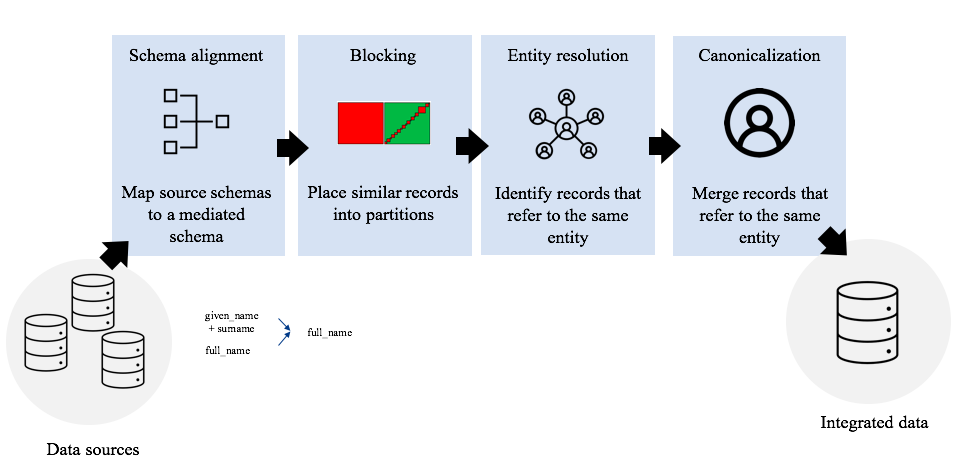
\includegraphics[scale=0.33]{finalFigures/pipeline}
%\caption{default}
%\label{default}
\end{center}
\end{figure}


}

\begin{frame}{Existing ER methods}
%  Common methods in statistics:\\
  \begin{enumerate}
   \item deterministic linking
   \item probabilistic linking (Fellegi Sunter, random forests, deep learning)
   \item Bayesian Fellegi Sunter 
  \end{enumerate}
  \pause

\vspace*{1em}
  Drawbacks:\\
  \begin{itemize}
    \setbeamertemplate{itemize item}{--}
%    \item pairs of records are assessed independently
%    \item awkward post-processing step (transitive closure)
    \item subjectivity in setting the decision threshold
    \item lack of uncertainty quantification
    \item require training data
%    \alert{\item scalability achieved via deterministic dimension reduction of the data}
  \end{itemize}
\vspace*{1em}
[Fellegi and Sunter (1969), Ventura et al. (2014), Christen (2012), Dong and Shrivastava (2015), Belin and Rubin (1995), Gutman et al. (2013), McVeigh et al. (2020), Sadinle (2014), Sadinle (2017), Sadinle (2018)]. 
\end{frame}

\frame{
\center
\Large

Graphical Entity Resolution

}

\frame{
\frametitle{Graphical Bayesian ER}

%\begin{itemize}
%\pause
%\item Dealing with big data means merging large, noisy databases.
%\pause
%\begin{itemize}
%\item Such databases have severe amounts of noise. 
%\end{itemize}
%\pause
%\item Entity resolution requires sophisticated graph structures. [Gutman et. al (2013)].
%\pause
%\begin{itemize}
%\item One approach is to use a bipartite graph for latent entities.
%\pause
%\item Never link records to records. 
%\pause
%\end{itemize}
%\item Computational speed-ups: eliminate low-probability matches.
%%\pause
%%\begin{itemize}
%%\item Blocking techniques based on locality-sensitive hashing.
%\end{itemize}
%\pause
Builds off Copas and Hilton (2001), Tancredi and Liseo (2011).

\begin{figure}[htbp]
\begin{center}
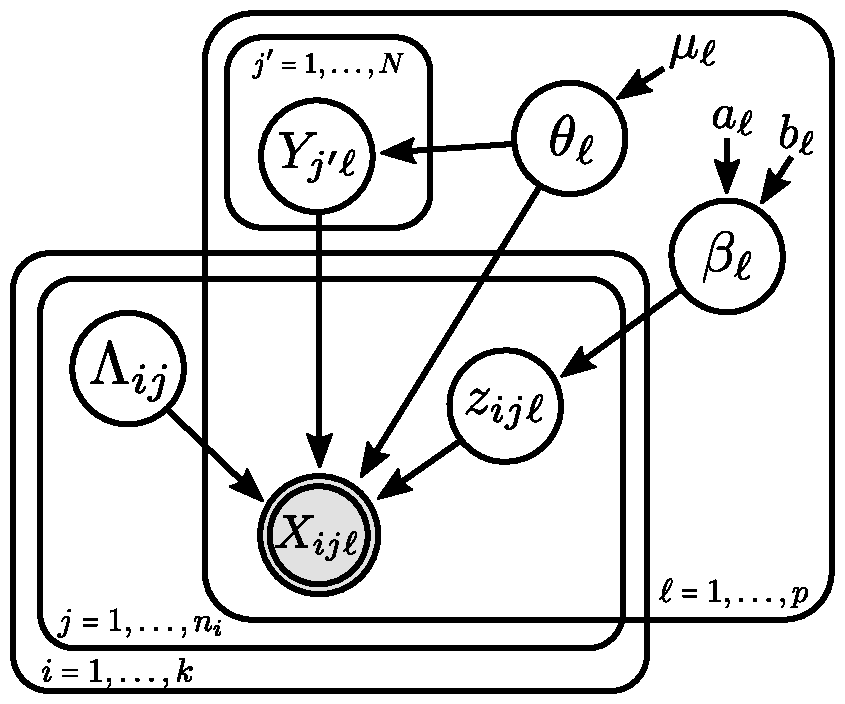
\includegraphics[width=0.5\textwidth]{finalFigures/recordLinkage_graphicalModel}
%\caption{Graphical representation of models \ref{model:cat}-\ref{model:string}.}
\label{fig:graphicalProcess}
\end{center}
\end{figure}

[Steorts+ 2014 AISTATS, Steorts+ 2016 JASA, Steorts 2015 BA]

}

\frame{
\frametitle{Why Graphical Bayesian ER}

\begin{enumerate}
\item Handles any number of databases simultaneously
\item Handles both categorical and textual data
\item Handles missing data 
\item Uncertainty quantification is natural 
\item Transitive closures are nearly free
\item Has sound theoretical properties 
\item Can scale to databases that contain millions of records
\item Generalizes to a wide variety of applications 
\item Has equivalent or better performance than alternatives
\item All software is open source and freely available to non-profits 
\end{enumerate}


}


\frame{

\begin{figure}[htbp]
\begin{center}
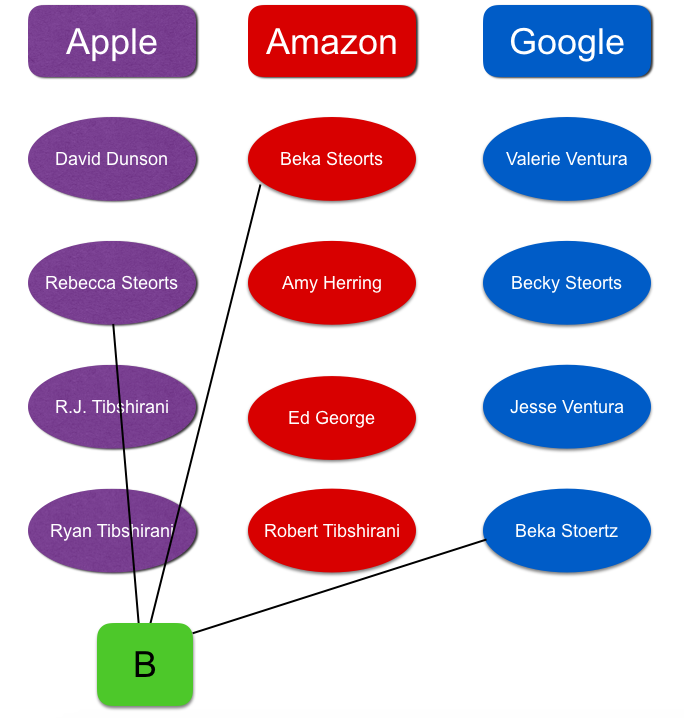
\includegraphics[width=0.7\textwidth]{pictures-new/latent-one}
%\caption{default}
%\label{default}
\end{center}
%\scriptsize{
%\begin{flushright}
%[Steorts, Hall, and Fienberg (2014), \emph{AIStats}.] \newline
%[Steorts, Hall, and Fienberg (2014), \emph{JASA}, In Revision.], [Steorts (2014), Submitted.] 
%\end{flushright}
%}
\end{figure}

}


\frame{

\begin{figure}[htbp]
\begin{center}
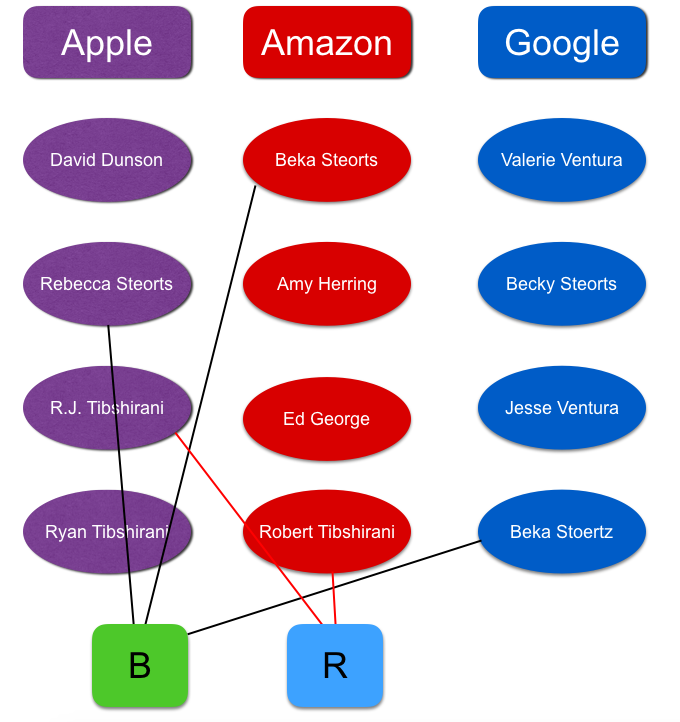
\includegraphics[width=0.7\textwidth]{pictures-new/latent-two}
%\caption{default}
%\label{default}
\end{center}
%\scriptsize{
%\begin{flushright}
%[Steorts, Hall, and Fienberg (2014), \emph{AIStats}.] \newline
%[Steorts, Hall, and Fienberg (2014), \emph{JASA}, In Revision], [Steorts (2014), Submitted.] 
%\end{flushright}
%}
\end{figure}

}







\frame{
\frametitle{Our Goal}
\center
\Large

To scale Bayesian ER methods to millions of records without  sacrificing accuracy
   and provide uncertainty of the ER task 

}




\frame{
\center
\Large

We propose a scalable joint (Bayesian) model for blocking and performing entity resolution, where the error from this joint task is measured exactly. 


}

\begin{frame}{Problem setup}
  \setlength{\leftmargini}{1.1em}
  \begin{columns}[onlytextwidth]
    \begin{column}{0.5\linewidth}
      Key assumptions:
      \begin{itemize}
        \item multiple tables\slash sources
        \item duplicates within and across tables
        \item attributes are aligned
        \item attributes are discrete
        \item some missing values
        \item no ground truth (unsupervised)
      \end{itemize}
    \end{column}
    \hfill
    \begin{column}{0.4\linewidth}
      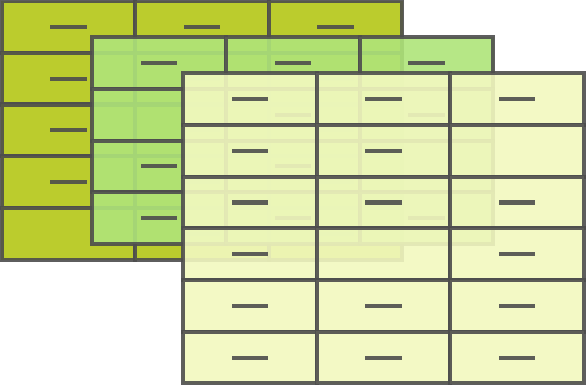
\includegraphics[width=\linewidth]{finalFigures/multiple-datasets.pdf}
    \end{column}
  \end{columns}
  \pause
  \bigskip

  Output: approximate posterior distribution over the linkage structure
\end{frame}



\frame{
\frametitle{Our contribution}



\begin{enumerate}
\item We propose a joint Bayesian model for blocking (latent entities) and entity resolution. 
\item We propose blocks (auxiliary partitions) that
induce conditional independencies between the latent entities. This enables distributed inference at the partition-level.
%, while crucially preserving the marginal posterior of the original model.
%\item Incorporating auxiliary partitions that
%induce conditional independencies between the entities. This enables distributed inference at the partition-level, while crucially preserving the marginal posterior of the original model. 
\item The blocking function (responsible for partitioning the entities) groups similar entities together while achieving well-balanced partitions.
\item Application of partially-collapsed Gibbs sampling in the context of distributed computing.
\item Improving computational efficiency:
\begin{enumerate}
\item[a)] Sub-quadratic algorithm for updating links based on indexing.
\item[b)] Truncation of the attribute similarities.
\item[c)] Perturbation sampling algorithm for updating the entity attributes, which relies on the Vose-Alias method.
\end{enumerate}
%	\item Auxiliary variable representation of the model 
%	(superclusters) that removes dependencies between some 
%	of the variables (enables parallel computing)
%	\item Novel ``perturbation'' discrete sampling algorithm 
%	(used to update $Y$)
%	\item Sub-quadratic algorithm for updating the links between records 
%	and latent entities 
%	\item Collapsed Gibbs sampler (updates $Y$ and partition assignments)
%	\item Re-parametrization for string attributes in terms of a 
%	truncated string similarity function
\end{enumerate}

[Marchant, Kaplan, Rubinstein, Elazar, Steorts (2021)]
}


\frame{
\frametitle{dblink}

\begin{figure}[htbp]
\begin{center}
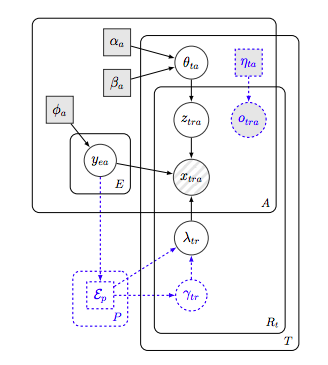
\includegraphics[scale=0.6]{finalFigures/dblink}
%\caption{default}
%\label{default}
\end{center}
\end{figure}

}

\section{Inference}
\begin{frame}{Distributed Markov chain Monte Carlo}
  Since the posterior for the linkage structure $p(\Lambda | X)$ is not 
  tractable, we resort to \alert{approximate inference}.
  \vspace*{1em}
  \pause

  We propose an MCMC algorithm based on the \alert{partially-collapsed Gibbs} 
  framework~(van Dyk and Park, 2008):
  \begin{itemize}
    \item regular Gibbs updates for the distortion probabilities $\theta_{ta}$, 
    distortion indicators $z_{tra}$ and links $\lambda_{tr}$
    \item ``marginalization'' and ``trimming'' are applied to jointly update 
    the entity attributes $y_{ea}$ and the partition assignments for the 
    linked records
    \item order of the updates is important (to preserve the stationary 
    distribution)
  \end{itemize}
\end{frame}

\begin{frame}{Distributed Markov chain Monte Carlo}
%  \begin{itemize}
%    \item Distribute inference using a master-worker architecture
%    \item Possible since records\slash entities are conditionally independent 
%    across partitions
%  \end{itemize}
  
  \begin{center}
    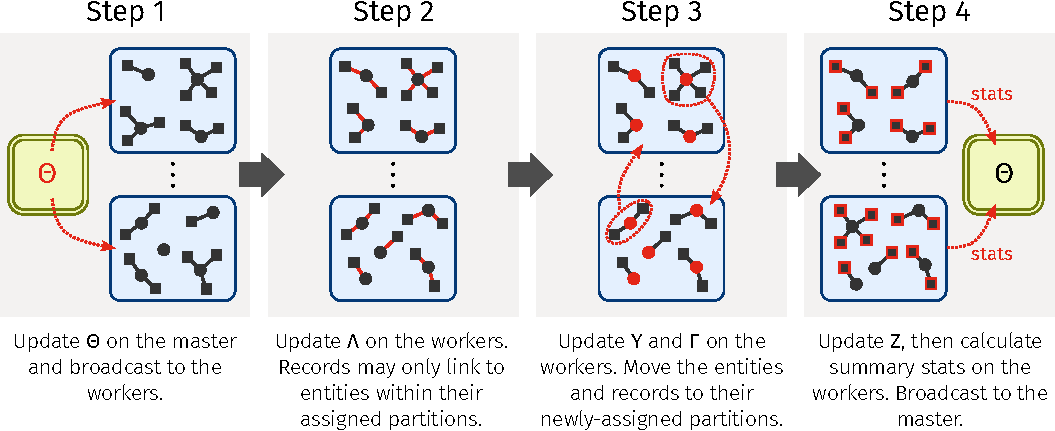
\includegraphics[width=\linewidth]{./figures/distributed-transition-operator.pdf}
  \end{center}
\end{frame}


\begin{frame}{Tricks for speeding up inference}
  Two main bottlenecks:
  \begin{enumerate}
    \item linkage structure update 
    $\mathcal{O}(\text{\# records} \times \text{\# entities})$ 
    \item entity attribute update 
    $\mathcal{O}(\text{\# entities} \times \text{domain size})$   \end{enumerate}
  
   \vspace*{2em}
   
  \pause
   Solutions:
   \begin{enumerate}
      \item Indexing: Maintain indices from ``entity attributes $\to$ entities'' and 
      ``entities $\to$ linked records." This allows us to prune candidate links for a record
   \item Thresholding similarity scores
    \item Express the distribution for the entity attribute update as a 
      two-component perturbation mixture model
   \end{enumerate}
   \end{frame}






\frame{
\frametitle{Experiments}

\begin{itemize}
  \item \texttt{ABSEmployee}. A synthetic data set used 
  internally for linkage experiments by the ABS.
%  It simulates an employment census and two supplementary 
%  surveys. 
  \item \texttt{NCVR}. Two snapshots from the North Carolina 
  Voter Registration database taken two months 
  apart. 
%  The snapshots are filtered to include only those voters 
%  whose details changed over the two-month period.
%  We use the full name, age, gender and zip code attributes.
  \item \texttt{NLTCS}. A subset of the National Long-Term 
  Care Survey comprising the 
  1982, 1989 and 1994 waves.
  %\footnote{A subset must be used as race was 
  %subsampled in the other three years, making it unsuitable for ER.}
  % NM-1: Removing this footnote purely to fix the layout.
  % RS: Okay. 
%  We use the SEX, DOB, STATE and REGOFF attributes.
  \item \texttt{SHIW0810}. A subset from the Bank of Italy's 
  Survey on Household Income and Wealth
  comprising the 2008 and 2010 waves.
  %\footnote{Available at \url{http://github.com/[REDACTED]}} 
%    We use 8 attributes: IREG, SESSO, ANASC, STUDIO, PAR, 
%  STACIV, PERC and CFDIC.
  % NM-1: The SHIW data set we used is _different_ to the one 
  % that appears in the italy R package.
  % The version we used is based on the raw data from the 
  % Bank of Italy website, with a correction to the NORD 
  % variable (done using an R script that I wrote).
  % I guess we could make this available on GitHub...
  % RS-1: Thanks for clarifying. Would be helpful to put on Github since they are different and there could be confusion with the two different versions. 
  
  \item \texttt{RLdata10000}. A synthetic data set provided 
  with the \texttt{RecordLinkage} R 
  package. % because all attributes are missing.
  % NM-1: This is not true. There are "non-missing" values 
  % in fname_c2 and lname_c2 for RLdata10000 
  % (you might be thinking of RLdata500?).
  % RS-1: Yes. Thank you, NM! 
\end{itemize}

}







\begin{frame}{Experiments}
  \begin{itemize}
    \item Implemented dblink and baselines in Apache Spark
    \item Ran experiments on a local server and Amazon EMR
    \item (Mostly) used a sample size of $10^3$ after burnin (of 
    $10^3$ iterations) and thinning (keeping every 10th iteration)
    \item 3 real and 2 synthetic data sets
  \end{itemize}
  \pause

  \begin{center}
    \footnotesize
    \begin{tabularx}{\linewidth}{l *{3}{c} *{2}{Y}}
      \toprule
      Data set & \# records & \# tables & \# entities & 
      \multicolumn{2}{c}{\# attributes} \\ 
      \cmidrule{5-6}
      & & & & {\footnotesize categorical} & {\footnotesize string } \\
      \midrule
      $\star$ \texttt{ABSEmployee} & 600,000 & 3 & 400,000 & 4 & 0 \\
      \texttt{NCVR}        & 448,134 & 2 & 296,433 & 3 & 3 \\
      \texttt{NLTCS}       &  57,077 & 3 &  34,945 & 6 & 0 \\
      \texttt{SHIW0810}    &  39,743 & 2 &  28,584 & 8 & 0 \\
      $\star$ \texttt{RLdata10000} &  10,000 & 1 &   9,000 & 2 & 3 \\
      \bottomrule
    \end{tabularx}
  \end{center}
\end{frame}


\frame{



\scriptsize{
\begin{table}
	\centering
	\caption{Assessment of the pairwise linkage performance for dblink and FS method as our baseline. We note that FS is supervised and does not propagate the entity resolution error exactly compared to dblink.}
	\vspace*{1em}
	\begin{tabular}{l l *{3}{c}}
		\toprule
		Data set    & Method & \multicolumn{3}{c}{Pairwise measure} \\
		\cmidrule(){3-5}
		 & & Precision & Recall & F1-score \\
		\midrule
		\multirow{2}{*}{\texttt{ABSEmployee}} 
		 & dblink                  & \textbf{0.9943} & \textbf{0.8867} & \textbf{0.9374} \\
		 & Fellegi-Sunter (100)  & {0.9964} & {0.9510} & {0.9736} \\
		 & Fellegi-Sunter (10)  & {0.4321} & {0.6034} & {0.9736} \\

		 
%		 & Near matching         & 0.0543 & \textbf{0.9970} & 0.1030 \\
%		 & Exact matching        & \textbf{0.9964} & 0.8849 & 0.9374 \\
		\midrule
		\multirow{2}{*}{\texttt{NCVR}}
		 & dblink                 & \textbf{0.9179} & \textbf{0.9654} & \textbf{0.9411} \\
		 & Fellegi-Sunter (100)  & 0.8989 & {0.9974} & {0.9456} \\
		 & Fellegi-Sunter (10)  & 0.8989 & {0.9974} & {0.9456} \\
%		 & Near matching         & 0.9899 & 0.7443 & 0.8497 \\
%		 & Exact matching        & \textbf{0.9925} & 0.0017 & 0.0034 \\
		\midrule
		\multirow{2}{*}{\texttt{NLTCS}}
		 & dblink                  & \textbf{0.8363} &  \textbf{0.9102} &  \textbf{0.8717} \\
		 & Fellegi-Sunter (100)  & 0.7969 & {0.9959} & {0.8853} \\
		  & Fellegi-Sunter (10)  & 0.1902 & {0.9999} & {0.3196} \\
%		 & Near matching         & 0.0385 & 0.9656 & 0.0740 \\
%		 & Exact matching        & \textbf{0.8451} & 0.9234 & 0.8825 \\ 
		\bottomrule
	\end{tabular}
\end{table}
}
\normalsize
[Marchant+ (2021) JCGS]
}

\frame{
\frametitle{Posterior Bias Plot}

\begin{figure}[htbp]
\begin{center}
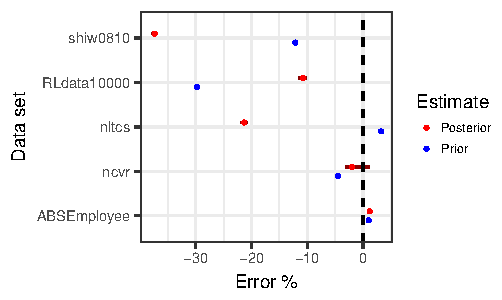
\includegraphics[scale=1]{figures/posterior-bias-plot}
\caption{Error in the posterior and prior estimates for the number of observed entities for d-blink. The results show that the posterior estimate is very sharp and typically underestimates the true number, which is consistent with Steorts, Hall, Fienberg (2016). }
\label{default}
\end{center}
\end{figure}

[Marchant+ (2021) JCGS]

}

\begin{frame}{Convergence of \dblink\ versus \blink}
  We examined the rate of convergence of \dblink\ versus \blink\ 
  on \texttt{RLdata10000} without partitioning.
  
  \begin{center}
    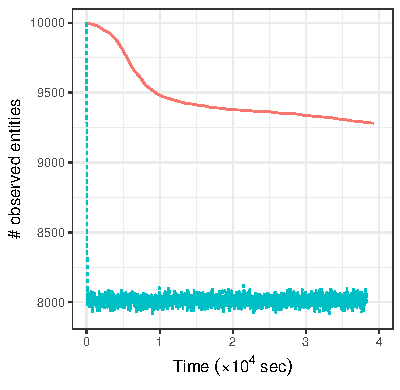
\includegraphics[height=0.45\textheight]{figures/convergence-num-ent-blink-dblink.pdf}
    \hfill
    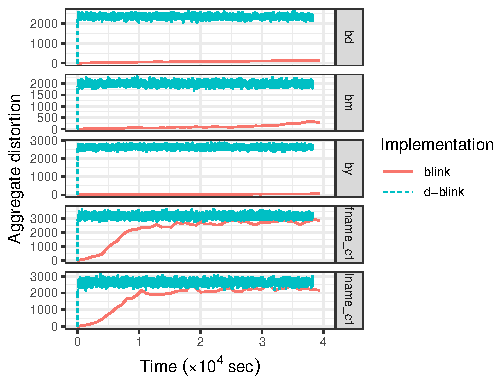
\includegraphics[height=0.45\textheight]{figures/convergence-agg-dist-blink-dblink.pdf}
  \end{center}

  \texttt{d-blink} converges rapidly, however \texttt{blink} fails to reach 
  the equilibrium distribution within 11 hours.
\end{frame}

\begin{frame}{Does partitioning result in efficiency gains?}
  \begin{itemize}
    \item Measure efficiency using \alert{ESS rate}---the effective sample 
    size generated per unit time
    \item \alert{Speed-up factor} is the ESS rate relative to a baseline 
    without partitioning
    \item Observe a near-linear speed-up for the \texttt{NLTCS} data set
    (tapering off beyond $\sim 20$ partitions)    
  \end{itemize}

  \begin{center}
    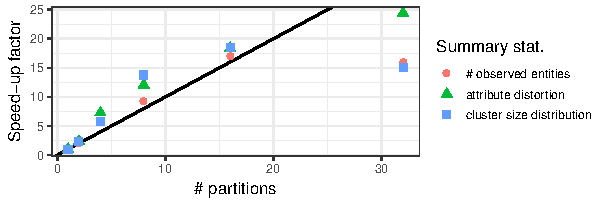
\includegraphics[width=0.9\textwidth]{figures/plot-partitions-speed-up-muppet.pdf}
  \end{center}
\end{frame}


\frame{
\frametitle{Case Study Applied to the 2010 Decennial Census}

\begin{table}
  \centering
  \caption{Results for ER of 2010 Census and Numident data in Wyoming. 
  Pairwise evaluation measures are computed using ground truth identifiers 
  available for a subset of the records, where the unadjusted count was reported to be 563,626.}
  \label{tbl:census-results}
  \footnotesize
  \begin{center}
  \begin{tabular}{*{3}{c} *{2}{c}}
    \toprule
    \multicolumn{3}{c}{Pairwise measures} & \multicolumn{2}{c}{Posterior population size} \\
    \cmidrule(lr){1-3} \cmidrule(lr){4-5}
    Precision & Recall & F1-score &    Mean & Std.~error \\
    \midrule
    0.97 &   0.84 &     0.90 & 616,000 & 5,000 \\
    \bottomrule
  \end{tabular}
  \end{center}
\end{table}

\vspace*{4em}

[Marchant+ (2021) JCGS]

}





\frame{
\center
Thank you! \\
Questions?\\

\vspace*{2em}
Contact: beka@stat.duke.edu\\
Webpage: resteorts.github.io\\
\vspace*{2em}

\href{https://arxiv.org/abs/2008.04443}{Binette and Steorts Review Article}\\
\href{https://github.com/orgs/cleanzr}{Entity Resolution Software}\\
\href{https://github.com/cleanzr/record-linkage-tutorial}{Entity Resolution Tutorial}\\


}









\end{document}